\documentclass[10pt]{article}
\usepackage{graphicx}
\usepackage{float} % to use [H] placement

\begin{document}
\section{Test Graphics}

\begin{center}
	\begin{figure}[H] %H means RIGHT HERE!
		%\includegraphics[width=0.4\linewidth]{images/ProbFunction} % to use images in a subdirectory
		\includegraphics[width=0.4\linewidth]{ProbFunction}
		\caption{Test Caption}
		\label{fig:TestLabel}
	\end{figure}
\end{center} 
We can see in \ref{fig:TestLabel} that blah blah.

%this seems to work better?
\begin{figure}[H] %H means RIGHT HERE!
	\centering
	\includegraphics[width=0.4\linewidth]{ProbFunction}
\end{figure}

\section{Multiple Images}
\begin{figure}[H] %H means RIGHT HERE!
	\centering
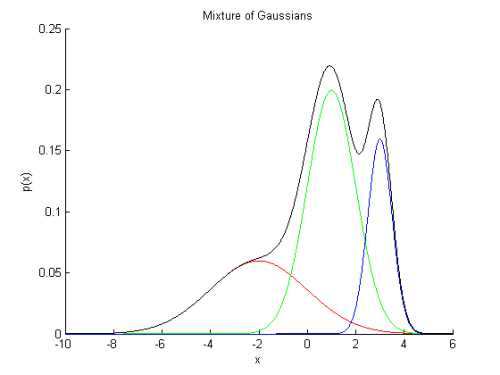
\includegraphics[width=0.4\linewidth]{Images/1}

\includegraphics[width=0.4\linewidth]{Images/2}
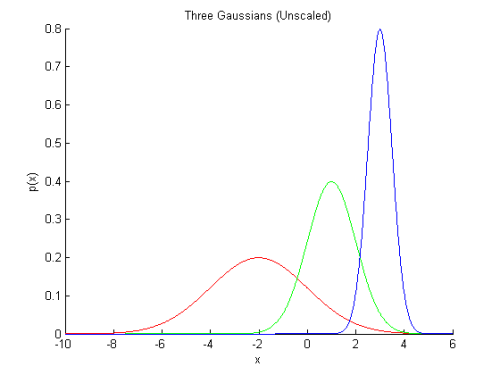
\includegraphics[width=0.4\linewidth]{Images/3}
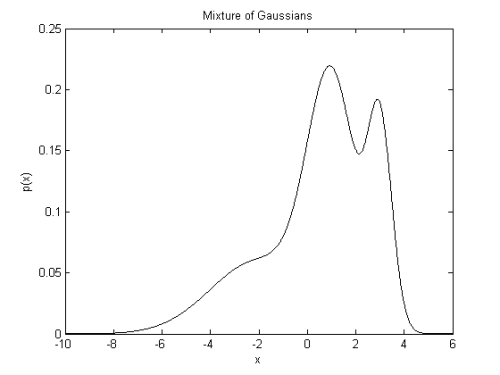
\includegraphics[width=0.4\linewidth]{Images/4}
\end{figure}

\section{Multiple Images (forced break}
\begin{figure}[H] %H means RIGHT HERE!
	\centering
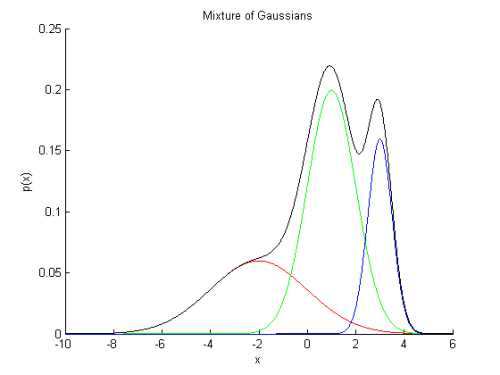
\includegraphics[width=0.4\linewidth]{Images/1}

\includegraphics[width=0.4\linewidth]{Images/2} \\ %sometimes you have to add this line break
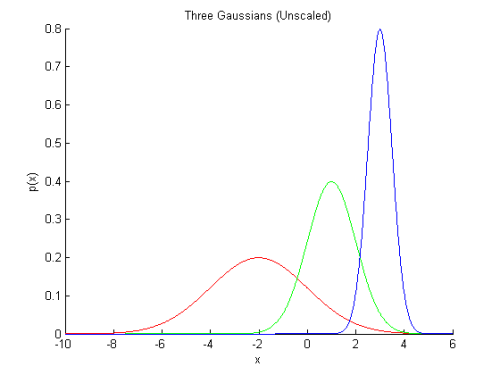
\includegraphics[width=0.4\linewidth]{Images/3}
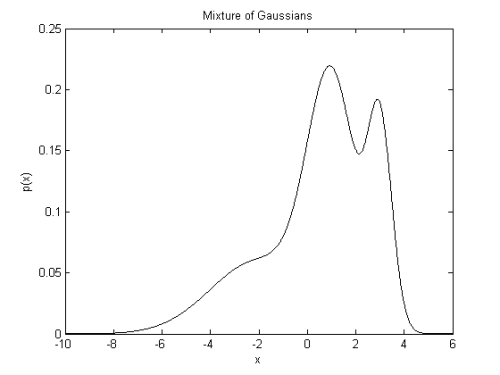
\includegraphics[width=0.4\linewidth]{Images/4}
\end{figure}

\end{document}
